\chapter[Railway conflict management]{Application to railway conflict management}
\label{chapter:trains}
As the last point in the thesis, in this chapter, we describe how the results
presented so far can be applied in the field of operational research. Namely,
we propose an approach to solving the railway dispatching problem using quantum
annealing. We benchmark the implementation of our algorithm on the current
generation of D-Wave annealers, using solutions obtained via tensor networks
and exhaustive search as a baseline for comparison.

\section{Overview of the problem}
We will consider a part of a railway network, which we will simply refer to as
a \emph{network}. The network is divided into \emph{block sections} or simply
\emph{blocks}. In our approach, we focused only on the single--track railways,
which means that the network can only comprise the following types of blocks:
\begin{itemize}
  \item \emph{Line blocks}, or \emph{single tracks}, sections that can be occupied by one train
    at a time.
  \item \emph{Sidings}, or \emph{parallel tracks} (occurring e.g. at stations). At the sidings,
    trains passing in the same direction can meet--and--overtake (M--O), and trains passing
    in the opposite directions can meet--and--pass (M--P). Each siding comprises two or more
    tracks, each of which can also be occupied by one train at a time. When appropriate, the
    sidings occurring at the stations will be called \emph{station blocks}.
\end{itemize}
Fig. \ref{fig:railway-network} shows an example network.

\begin{figure}[ht]
  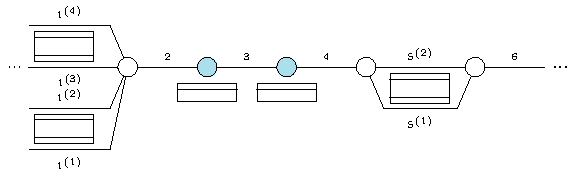
\includegraphics[width=\textwidth]{figures/example_line}
  \caption{
    An example network. Sections $2, 3, 4$ and $6$ are \emph{line blocks}, while
    sections $1$ and $5$ are \emph{sidings} with respectively $4$ and $2$ tracks.
    Rectangles represent platforms. Circles represent points where a line block and
    a siding join (white) or where two line blocks join (blue). Superscripts denote
    tracks within a siding. } \label{fig:railway-network}
\end{figure}

The trains move through the network according to a \emph{timetable}. It is
assumed that this timetable is conflict-free, i.e. at any time no two trains
occupy the same track.

Now, suppose the network is affected by a disturbance, which has prevented some
trains from running according to their original timetable. Examples of possible
disturbances include, but are not limited to, a malfunction of one or more
trains or a malfunction of railway tracks. After the disturbance, some trains
occupy different parts of the networks than they are supposed to and resuming
operations according to the original timetable might not be possible. First of
all, some trains might already be delayed too much to be physically able to
follow the timetable. Secondly, trying to closely follow the timetable after
the disturbance might generate conflicts. The problem might be viewed from
various perspectives, e.g. that of a passenger or transport operation company
\cite{tornquist,lamorgese,Jensen2016}. This this chapter, we look at the
problem of the infrastructure manager whose task, in the presence of a
disturbance, is to create a new, conflict-free timetable. Naturally, in most
cases, there will be multiple possible solutions to the arising conflicts, and
hence one has to decide on what criteria make one timetable more appealing than
another. In our approach, we assume that the dispatcher aims to minimize some
function of the delays, which we will describe later. There are also other
possible choices of the objective function \cite{8795577} such as the total
passenger delay or the total cost of operations.

Let us observe that independently from the algorithm for constructing a new
timetable, some delays after the disturbance might be inevitable, e.g. due to
engineering or even physical limits. For instance, if a train has been broken
for some time, it can only follow the timetable if it is not already late and
it can make up for the time it already lost -- and this can only happen if it
can reach a sufficiently large speed. If this is not the case, the train will
be necessarily delayed. Moreover, by taking into account the maximum speed with
which the trains can move through each section, one can calculate the lower
bounds on how much the train will be delayed at each station. These lower
bounds are known as unavoidable, or \emph{primary}, delays.

In the ideal case, if all the trains could travel at their maximum speed, all
trains would be delayed only by their primary delays and there would be nothing
to optimize. However, it might not always be possible. Suppose for instance,
that two trains going in the same direction are already delayed at a station
neighboring a line block. From each train's perspective, the optimal solution
is to start its route immediately when possible. However, as only one of them
can do this because a line block can only be occupied by one train at a time.
Hence, at least one of these two trains will have a delay larger than the
primary one. What is important is that this additional delay is not a
consequence of some physical or engineering limitations, but rather a
consequence of the dispatcher's decision made to avoid a potential conflict.
All such delays are called the \emph{secondary} delays and, unlike the primary
ones, they are subject to optimization.

The distinction between primary and secondary delays might seem artificial at
first, but it has profound consequences. Namely, when constructing a function
to be minimized we only need to take into account the secondary delays. For
instance, we might want to minimize their total sum or their weighted sum, with
weights corresponding to the trains' priorities.

Our high--level description of the problem needs now a mathematical
formulation. We start by describing the details of the network model in the
next section.

\section{The delay representation}
Before we can formulate the optimization problem to be run on D-Wave, we need
first to formally describe the railway model. The first idea that comes to mind
is to define quantities corresponding to departure and arrival times of each
train and relevant station blocks, and express all other quantities in the
model in terms of their difference with respect to the times found in the
original timetable. However, as we will soon see, one can almost completely
forget about arrival and departure times, and instead express all qunatities in
the model using delays. Moreover, we will further simplify our model by
assuming all secondary delays are integers falling into some finite range.

The set of all trains will be denoted by $\JJ$. This set is naturally
partitioned into the set $\JJ_0$ of trains going into one direction and the set
$\JJ_1$ of trains going into the opposite direction. This is a proper
partition, i.e.:
\begin{equation}
  \JJ_0 \cup \JJ_1 = \JJ \quad \JJ_0 \cap \JJ_1 = \emptyset
\end{equation}
For any train $j \in \JJ$ its route is a sequence of blocks. Our model forbids
recirculation, i.e. each train passes every block in its route exactly once.
Furthermore, we assume that each train starts and ends its route at some
station, and its route is uniquely identified by a sequence of station blocks
$\left(s_{j,1}, s_{j, 2}, \ldots, s_{j, \text{end}_j}\right)$, i.e., there are
no alternative routes between any two stations. For convenience, we will denote
the station block preceding $s_{j,k}$ in a given train's route by
$\pi(s_{j,k})$ and the station block succeeding it by $\rho(s_{j,k})$:
\begin{align}
  \pi(s_{j,k})  & = s_{j,k-1} \quad \mbox{for } 2 \le k \le \mbox{end}_j      \\
  \rho(s_{j,k}) & = s_{j,k+1} \quad \mbox{for } 1 \le k \le \mbox{end}_j - 1.
\end{align}
We will denote the time at which the train $j$ should leave the block $s$
according to the original timetable by $\ttout(j, s)$. Similarly, the time at
which the train $j$ is supposed to leave block $s$ will be denoted by $\ttin(j,
  s)$. In our model, we assume that the time at which a train leaves one block is
precisely the same as the time it enters the next block, i.e.
\begin{equation}
  \ttout(j, s) = \ttin(j, \rho_j(s))
\end{equation}
It is clear that the original timetable determines how long it takes for a
train $j$ to travel through a given block $s$. We call this time the passage
time, denoted by $\pt(j, s)$
\begin{equation}
  \pt(j, s) = \ttout(j, s) - \ttin(j, s)
\end{equation}
An important observation is that passage times defined by the timetable may not
be the minimum physically achievable passing times $\pmin(j, s)$. In other
words, for each train $j$ and block $s$ there exists a time reserve
\begin{equation}
  \label{eq:pt}
  0 \le \alpha(j, s) = \pt(j, s) - \pmin(j, s)
\end{equation}
This time reserve will become important when discussing the propagation of the
primary delays.

\subsection{Delay representation}
Suppose the disturbance happened, resulting in some trains not being able to
meet the schedule. Hence, the actual leaving and arrival times (denoted by
$\tout$ and $\tin$) differ from the scheduled ones. The delay $d(j, s)$ of the
train $j$ at block $s$ is defined as the difference
\begin{equation}
  \label{eq:djs}
  d(j, s) \coloneqq \tout(j, s) - \ttout(j, s) %= \tin(j, \rho(s)) - \ttin(j, \rho(s)).
\end{equation}
As already mentioned, $d(j, s)$ can be expressed as a sum
\begin{equation}
  d(j, s) = d_U(j, s) + d_S(j, s)
\end{equation}
where $d_U$ denotes the primary (or unavoidable) delay, and $d_S$ denotes the
secondary delay. In the absence of time reserve, one would simply have $d_U(j,
  s) = d_U(j, s')$ for a given train $j$ and blocks $s$ and $s'$ on its route.
However, the time reserve allows to somewhat compensate the delays
\begin{equation}
  d_U(j, \rho(s)) = \max\{0, d_U(j, s) - \alpha(j, \rho(s))\}
\end{equation}

The secondary delays can be, in principle, arbitrary large. However, it is
convenient to assume that all secondary delays for the train $j$ are bound from
above by some constant $d_{\max}(j)$. One can find a reasonable upper bound by
running some fast heuristic or determine it manually (e.g. there might be an
\emph{a priori} established maximum allowable delay of the train). Henceforth,
we will consider $d_{\max}(j)$ to be a parameter of the model. With this
assumption, we have the following upper and lower bound on the overall delay
\begin{equation}
  d_U(j, s) \le d(j, s) \le d_U(j, s) + d_{\max}(j).
\end{equation}

\section{Discretizing delays}
Formulation of the problem presented so far can facilitate the construction of
a linear, constrained model of the dispatching problem. However, since the
secondary delay values are continuous variables, such a model would not be
compatible with the quantum annealer. We circumvent this issue by discretizing
the delays. One way to do it is to require that all secondary delays are
natural numbers, i.e.
\begin{equation}
  \forall_{j \in \JJ} \forall_{s \in S_{j}}\quad  d_{s}(j, s) \in \{0, 1, \ldots, d_{\max}(j)\}.
\end{equation}
As a consequence, the total delays get discretized as well. We will denote the
set of possible values for $d(j, s)$ by $A_{j, s}$, i.e.
\begin{equation}
  A_{j, s} \coloneq \{d_{U}(j, s), d_{U}(j, s) + 1, \ldots, d_{U}(j, s) + d_{\max}(j)\}.
\end{equation}
Notice that this discretization is not particularly restrictive, as timetables
typically have a finite resolution of minutes anyway.

We can now use one--hot encoding for $d(j, s)$ and introduce binary variables
$x_{s, j, m}$:

\begin{equation}
  \forall_{j \in \JJ}\forall_{s \in S_{j}} \forall_{m \in A_{j, s}} \quad x_{s,j,m} = \begin{cases}
    1, & d(j, s) = m      \\
    0, & \mbox{otherwise}
  \end{cases}.
\end{equation}
Naturally, possible values for $d(j, s)$ are mutually exclusive, which can be
expressed as the following constraint:
\begin{equation}
  \label{eq:onehotconstraint}
  \forall_{j \in \JJ}\forall_{s \in S_{j}} \sum_{m \in A_{j, s}} x_{s, j, m} = 1
\end{equation}
As for the cost function, we decided to use a simple weighted sum of the
delays, i.e. the cost function of the form
\begin{equation}
  \label{eq:qubo:cost}
  f(\mathbf{x}) = \sum_{j \in \mathcal{J}}\sum_{s \in S^{*}_{j}}\sum_{m \in A_{j,s}} w(s,j,m) \cdot x_{j,s,m},
\end{equation}
For instance, choosing $w(s, j, m)=m$ would result in an objective of
minimizing the sum of all delays. In general, however, one could take into
account the relative importance of the trains, as we will describe later when
introducing the real railway sections considered in our research.

\section{Dispatching conditions}
The cost function \eqref{eq:qubo:cost} together with constraint
\eqref{eq:onehotconstraint} is not enough to construct a meaningful
optimization problem. We also have to take into account other constraints
stemming from dispatching conditions. For instance, we cannot allow a schedule
in which two trains occupy the same track at the same time. We will address
these additional dispatching conditions next.

\subsection{The minimum passing time condition.}
Train cannot travel through a block faster than the corresponding minimum
passing time
\begin{equation}
  \label{eq:dc1}
  \tout(j, s) \ge \tin(j, s) + \pmin(j, s).
\end{equation}
Using \eqref{eq:djs} and \eqref{eq:pt} one can easily verify that inequality
\eqref{eq:dc1} is equivalent to
\begin{equation}
  \label{eq:passingtime}
  d(j, \rho(s)) \ge d(j, s) - \alpha(j, s, \rho(s)).
\end{equation}
In binary variables, it means that if, for a fixed $j,s,m$, the $x_{j,s,m}=1$,
then delays $d(j,s)$ smaller than $m-\alpha(j, s, \rho_j(s))$ are prohibited
and thus the corresponding variables have to zero-out. Hence, we arrive at the
following condition:
\begin{equation}
  \label{eq:qubo:passingtime}
  \forall_{j} \forall_{s \in S_j \setminus \{s_{{j,\text{end}}}\}}
  \sum_{d \in A_{j,s}}
  \left(
  \sum_{ d' \in D(d) \cap A_{j, \rho_j(s)}} x_{j, s, d}
  x_{j, \rho_j(s), d'} \right) = 0,
\end{equation}
where $D(d) = \{0, 1, \ldots, d - \alpha(j, s, \rho_j(s)) -1\}$.
\subsection{The single block occupation condition.}
Two trains cannot occupy the same part of a single railway track. Consider two
trains, $j, j' \in \JJ_0$ leaving the same station $s$ in the direction of the
next station block $\rho_j(s)$. Suppose further that the train $j$ leaves
first. i.e. $\tout(j', s) > \tout(j, s)$. Since two trains cannot occupy the
same block, some amount of time has to pass after $\tout(j, s)$ before the
train $j'$ can leave. This amount of time is dependent on both $j$ and a
sequence of blocks, and hence we denote it by $\tauu(j, s, \rho_j(s))$. Thus,
the condition becomes
\begin{equation}
  \label{eq:single-block}
  \tout(j', s) \ge \tout(j, s) + \tauu(j, s, \rho_j(s)).
\end{equation}
Substituting for $\tout$ in \eqref{eq:single-block} yields the following
inequality for delays
\begin{equation}
  \label{eq:single-block-delays}
  d(j', s) \ge d(j, s) + \ttout(j, s) - \ttout(j', s) + \tauu(j, s, \rho_j(s))
\end{equation}
or,
\begin{equation}
  d(j', s) \ge d(j, s) + \Delta(j, s, j', s) + \tauu(j, s, \rho_j(s))
\end{equation}
where
\begin{equation}
  \label{eq:delta}
  \Delta(j, s, j', s) = \ttout(j, s) - \ttout(j', s)
\end{equation}
The precise form of $\tauu$ depends on the dispatching detail of the problem.
In our approach, we propose the following form:
\begin{equation}
  \tauu(j, s) = \max_{i \in \{k+1,\ldots,l-1\}}(\ttin(j, m_{i+1}) - \ttin(j, m_i))
\end{equation}

For our decision variables, we use a similar scheme as with the previous
constraint, and the condition becomes:
\begin{equation}
  \label{eq:qubo:singleblock}
  \forall_{i=0,1} \forall_{j, j' \in \JJ^{i}} \forall_{s \in S^{*}_{j} \cap S^{*}_{j'}} \sum_{m \in A_{j, s}} \left(
  \sum_{m' \in B(m) \cap A_{j', s}} x_{j,s,m}x_{j',s,m'}
  \right) = 0,
\end{equation}
where $B(m) = \{m + \Delta(j, s, j', s), d + \Delta(j, s, j', s)+ 1,\ldots, m +
    \Delta(j, s, j', s) + \tau_{(1)}(j,s, \rho_j(s))-1 \}$ is a set of delays
violating condition \eqref{eq:single-block-delays}.

\subsection{The deadlock condition}
The deadlock condition is analogous to the single block occupation condition
but for trains going in opposite directions. Suppose trains $j$ and $j'$ are
heading in opposite directions on a route determined by two consecutive
stations $s$ and $\rho_j(s)$. Note that for $j'$ the order is reversed, i.e. it
starts at $\rho_j(s)$ and travels in the direction of $s$. In this case, $j$
has to arrive at $\rho_j(s)$ before $j'$ can leave $\rho_j(s)$. We formalize it
as:
\begin{equation}
  \label{eq:deadlock}
  \tout(j', \rho_j(s)) \ge \tout(j,s) + \tauuu(j, s, \rho_j(s)),
\end{equation}
where $\tauuu(j, s, \rho_j(s))$ is the minimum time required for train $j$ to
get from station block $s$ to $\rho_{j}(s)$. Rewritten in terms of delays, the
inequality \eqref{eq:deadlock} reads:
\begin{equation}
  \label{eq:deadlock2}
  d(j',\rho_j(s)) \ge d(j, s) + \Delta(j,s,j',\rho_j(s)) + \tauuu(j, s, \rho_j(s)).
\end{equation}
This condition is to be applied for pairs of trains $j,j'$ going in opposite
dimension if train $j$ is supposed to leave before the train $j'$ leaves
$\rho_{j}(s)$, otherwise the order has to be appropriately reversed.

In decision variables, the deadlock condition in its basic form looks as
follows
\begin{equation}
  \label{eq:qubo:deadlock}
  \forall_{s \in S^{*}_{j} \cap S^{*}_{j'}} \sum_{m \in A_{j, s}} \left(
  \sum_{m' \in C(m) \cap A_{j', s}} x_{j,s,m}x_{j',s,m'}
  \right) = 0,
\end{equation}
and has to be applied for limited number of trains $j \in \JJ^{0} (\JJ^{1})$
and $j' \in \JJ^{1}(\JJ^{0})$. This limit is imposed indirectly by the upper
bounds on the delays. Here, $C(m)$ is, similarly to $B(m)$, the set of delays violating
the condition for the given pair.
\subsection{The rolling stock circulation condition}
Our model assumes that some trains are assigned the same train set. Naturally,
there exists some necessary \emph{turnover time}, before a train set can be
used. Formally, if trains $j$ and $j'$ going in opposite directions are
assigned the same train set, then the following inequality has to hold:
\begin{equation}
  \tout(j', s_{j',1}) > \tout(j, s_{j,end}) + \Delta(j, j')
\end{equation}
where $\Delta(j, j')$ is the minimum turnover time. In the delay
representation, the inequality becomes:
\begin{equation}
  \label{eq:rolling}
  \begin{split}
    d(j',s_{j',1}) + \ttout(j',s_{j',1}) > & \; d(j, s_{j,end-1}) + \ttout(j, s_{j,end-1}) + \\
    & \; \tauuu(j, s_{j,end-1}) + \Delta(j,j').
  \end{split}
\end{equation}
Inequality \eqref{eq:rolling} can be simplified to
\begin{equation}
  d(j',s_{j',1}) > d(j, s_{j,end-1}) - R(j,j'),
\end{equation}
by setting
\begin{equation}
  \label{eq:rolling2}
  R(j, j') = \ttout(j',s_{j',1}) - \ttout(j, s_{j,end-1}) - \tauuu(j,s_{j,end-1})
\end{equation}
In decision variables, the rolling stock circulation condition for trains $j$
and $j'$ can be written as
\begin{equation}
  \label{eq:qubo:rollingstock}
  \sum_{m \in A_{j, s_{(j, end-1)}}} \sum_{m' \in E(d) \cap A_{j',s_{(j',1)}}} x_{j,s_{(j,end-1)},m}x_{j', s_{(j',1)},m'} = 0
\end{equation}
where $E(d) = \{0, 1, \ldots, m-R(j, j')\}$.

\subsection{Penalties}
The conditions \eqref{eq:qubo:passingtime}, \eqref{eq:qubo:singleblock},
\eqref{eq:qubo:deadlock}, \eqref{eq:qubo:rollingstock} together with cost
function \eqref{eq:qubo:cost} define a constrained $0-1$ problem. However, in
order to use a quantum annealer, we must convert it to QUBO, which means we have to
incorporate those constraints into the cost function.

One might observe that penalties defined by the dispatching conditions are of
the form:
\begin{equation}
  \label{eq:quadraticpenalty}
  \sum_{(j, j') \in \mathcal{V}_{p}} x_{i}x_{j} = 0,
\end{equation}
for some set of pairs of indices $\mathcal{V}_{p}$. For every feasible solution
(i.e. one meeting all the constraints) the sum in equation
\eqref{eq:quadraticpenalty} is 0, whereas violation of the corresponding
condition gives a strictly positive value. Hance, one can add such a sum to the
cost function, effectively penalizing the infeasible solutions. More generally,
one might multiply the sum by some constant $p_{pair} > 0$, to further
increase the value of the cost function for the infeasible solutions.

The same reasoning cannot be applied e.g. to the constraint
\eqref{eq:onehotconstraint}, which comprises equations of the form
\begin{equation}
  \label{eq:linearpenalty}
  \sum_{i \in \mathcal{V}_{s}}x_{i} = 1.
\end{equation}
If one added sums from the equation \eqref{eq:linearpenalty} to the cost
function, it would favor the infeasible solution comprising of all 0s. Instead,
one can consider the following quadratic form of the same penalty:
\begin{equation}
  \label{eq:linearpenalty2}
  \left(\sum_{i \in \mathcal{V}_{s}}x_{i} -1 \right)^{2} = 0
\end{equation}
In contrast to \eqref{eq:linearpenalty}, this time the left hand is equal to 0
for feasible solution, and a positive value for any solution violating the
one--hot encoding constraint. As with previous, quadratic penalties, we might
want to multiply such penalties by some constant $p_{sum} > 0$. An important
thing to mention here is that the expansion of the left-hand side in
\eqref{eq:linearpenalty2} gives a nonzero constant offset, which we will
ignore. therefore, the final form of the penalty term reads:
\begin{equation}
  \mathcal{P}_{sum}(\mathbf{x}) = \sum_{\mathcal{V}_{s}}p_{sum}\left(\sum_{i,j \in \mathcal{V}_{s}^{\times 2}, i\ne j} x_{i}x_{j}  - \sum_{i \in \mathcal{V}_{s}}x_{i}\right).
\end{equation}
Lastly, the total cost function for our QUBO reads:
\begin{equation}
  f'(\mathbf{x}) = f(\mathbf{x}) + \mathcal{P}_{sum}(\mathbf{x}) + \mathcal{P}_{pair}(\mathbf{x}).
\end{equation}
\section{Results}

\subsection{Studied railway segments}
In our work, we considered two single-track railway lines managed by the polish
state--owned company PKP Polskie Linie Kolejowe:

\begin{itemize}
  \item Railway line No. 216 (Nidzica -- Olsztynek section)
  \item Railway line No. 191 (Goleszów -- Wisła Uzdrowisko section)
\end{itemize}

The segments are depicted in Fig. \ref{fig:linesmall:line} and Fig.
\ref{fig:linelarge:line}. For the railway line No. 216, we considered its
official train schedule (as of April 2020). The line No. 191 was undergoing a
renovation at the time of writing, and hence it had no available timetable.
Based on the planned parameters of the line, as described in the official
documents \cite{PKPPLK}, we constructed a cyclic timetable. Initial,
undisturbed timetables are depicted in Fig. \ref{fig:linesmall:diagram} and
Fig. \ref{fig:linelarge:diagram}.

\begin{figure}
  \begin{subfigure}{\textwidth}
    \caption{}\label{fig:linesmall:line}
    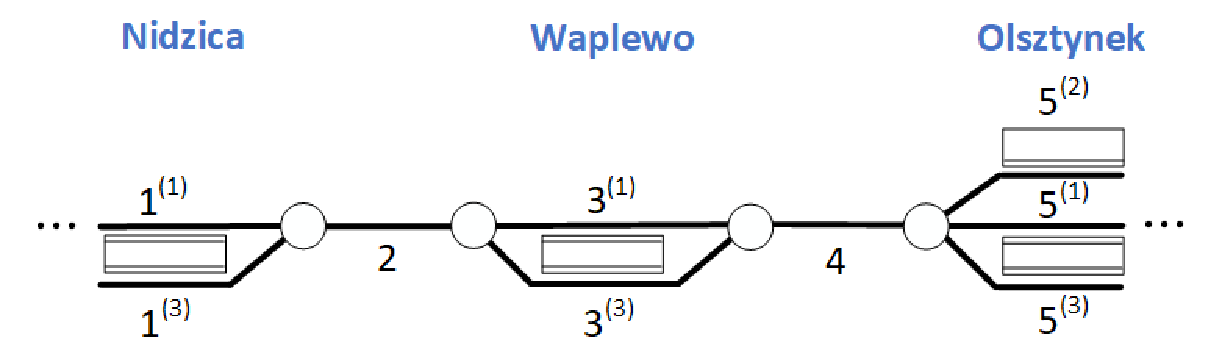
\includegraphics[width=\textwidth]{figures/line_small.pdf}
  \end{subfigure}
  \begin{subfigure}{\textwidth}
    \caption{}\label{fig:linesmall:diagram}
    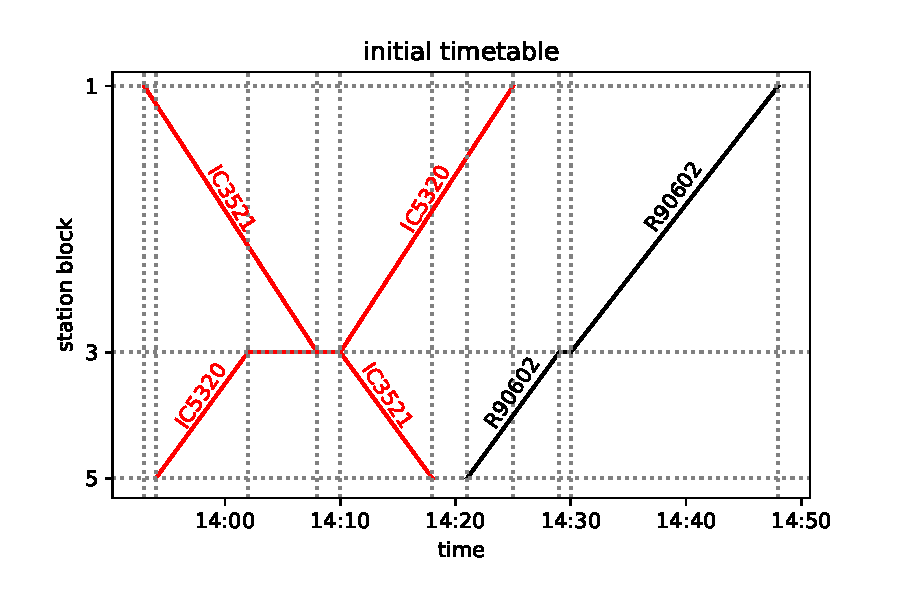
\includegraphics[width=\textwidth]{figures/train_diagram_small}
  \end{subfigure}
  \caption{\subref{fig:linesmall:line} Nidzica -- Olsztynek segment of line No. 216. The segment comprises three
    station blocks (1 -- Nidzica, 3 -- Waplewo, 5 -- Olsztynek), and two line
    blocks (2, 4). We assume that passing through the station block takes the same
    amount of time independently of which track is used. \subref{fig:linesmall:diagram} Train diagram for the undisturbed timetable of the line in \subref{fig:linesmall:line}. The timetable features two
    \emph{Inter--City} trains IC3521 and IC3520 and one \emph{Regio} train R90602. The paths for the
    \emph{Inter-City} trains are marked with red and path of the \emph{Regio} train is marked with black.}
  \label{fig:linesmall}
\end{figure}

\begin{figure}
  \begin{subfigure}{\textwidth}
    \caption{}\label{fig:linelarge:line}
    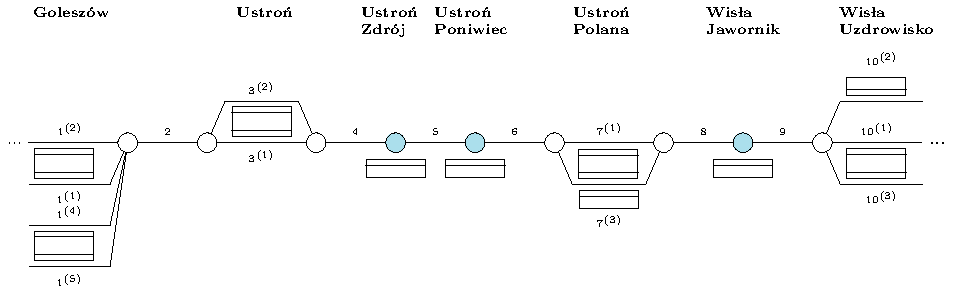
\includegraphics[width=\textwidth]{figures/line.pdf}
  \end{subfigure}
  \begin{subfigure}{\textwidth}
    \caption{}\label{fig:linelarge:diagram}
    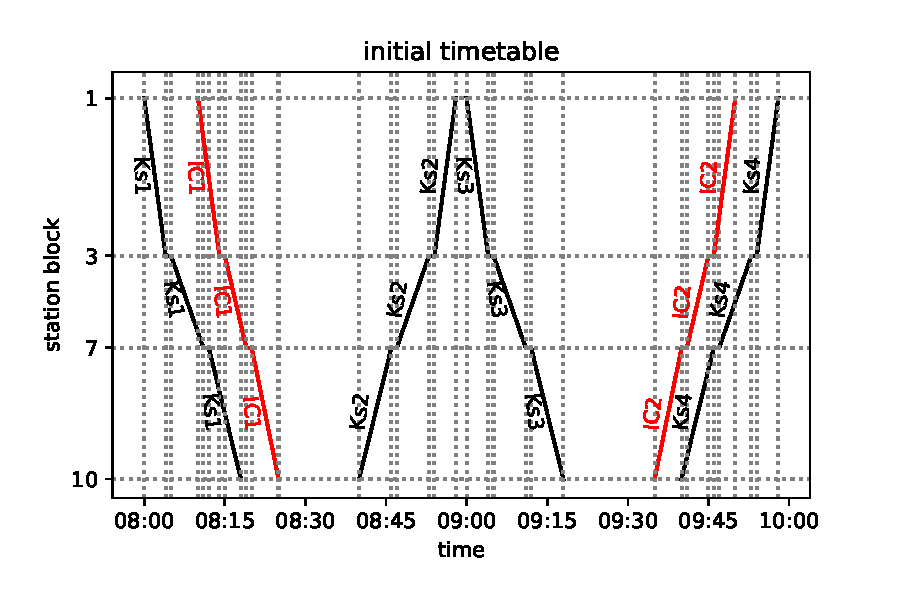
\includegraphics[width=\textwidth]{figures/train_diagram}
  \end{subfigure}
  \caption{\subref{fig:linelarge:line} Goleszów -- Wisła Uzdrowisko segment of line No. 191. The segment comprises 4
    station blocks (1 -- Goleszów, 3 -- Ustroń, 7 -- Ustroń Polana, 10 -- Wisła
    Uzdrowisko) and 6 line blocks (2, 4, 5, 6, 8, 9). Between line blocks there are
    additional passenger platforms at Ustroń Zdrój, Ustroń Poniwiec and Wisła
    Jawornik. \subref{fig:linelarge:diagram} Train diagram for the timetable of the line in \subref{fig:linelarge:line}.
    The timetable features two \emph{Inter--City} trains (IC1 and IC2) and four regional trains (Ks1--Ks4).
    The paths of the \emph{Inter--City} trains are marked with red and paths of the regional trains are
    marked with black.}
  \label{fig:linelarge}
\end{figure}

Timetable for the network segment of line No. 216 includes two
\emph{Inter-City} trains, IC5320 and IC3521, and a regional \emph{Regio} train
R90602. For the line No. 191, the timetable includes two \emph{Inter-City}
trains IC1, IC2 and four regional trains Ks1--Ks4. We assume both
\emph{Inter-City} trains in line No. 191 are operated with the same train set,
with a minimum service time of $R(j,j') = 20\mbox{minutes}$.

For both network segments, we assume that the minimum waiting times at all
considered stations are 1 minute. Also, we assume that the passing times
through all the line blocks were initially scheduled according to the maximum
permissible speeds. As a result of those assumptions, the only possible nonzero
time reserve occurs at the station blocks.

\subsection{Disturbance scenarios}

For the Nidzica--Olsztynek railway segment, we considered a single scenario
with two delays. The purpose of this scenario is to illustrate our approach on
a simple and yet real-world example. The first one is a 15-minute delay of
IC5320 starting from station block 5. The second one is that of the IC3521
leaving station block 1 5 minutes late. Considering this and our assumptions,
this creates conflicts, where two \emph{Inter--City} trains, as well as an
\emph{Inter--City} train and the \emph{Regio} train, have conflicts at block 4.
The conflicted, infeasible train diagram for this situation is depicted in Fig.
\ref{fig:smallconflict}.

\begin{figure}
  \begin{subfigure}[b]{0.5\columnwidth}
    \caption{}\label{conflict}
    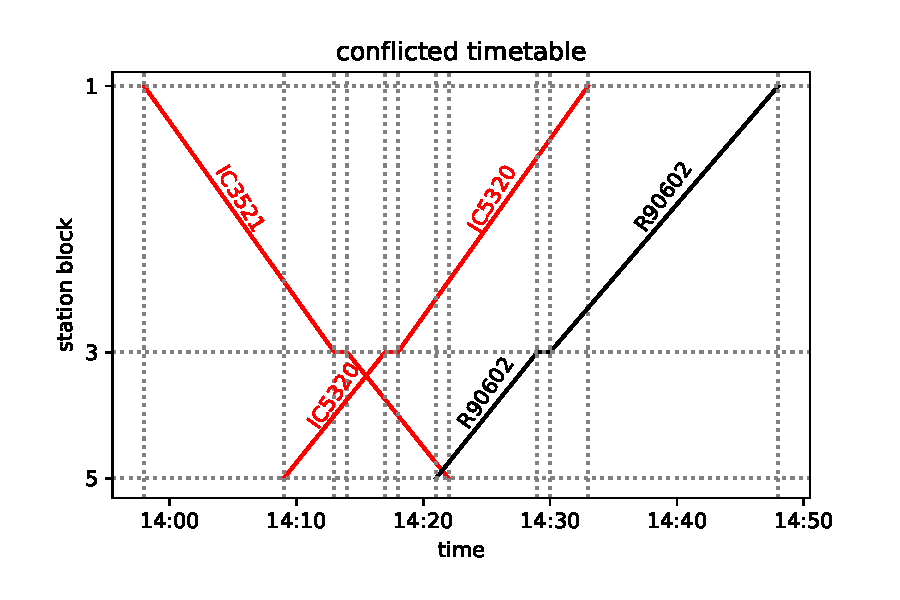
\includegraphics[width=\textwidth]{figures/small_conflict}
  \end{subfigure}
  \begin{subfigure}[b]{0.5\columnwidth}
    \caption{}\label{resolution}
    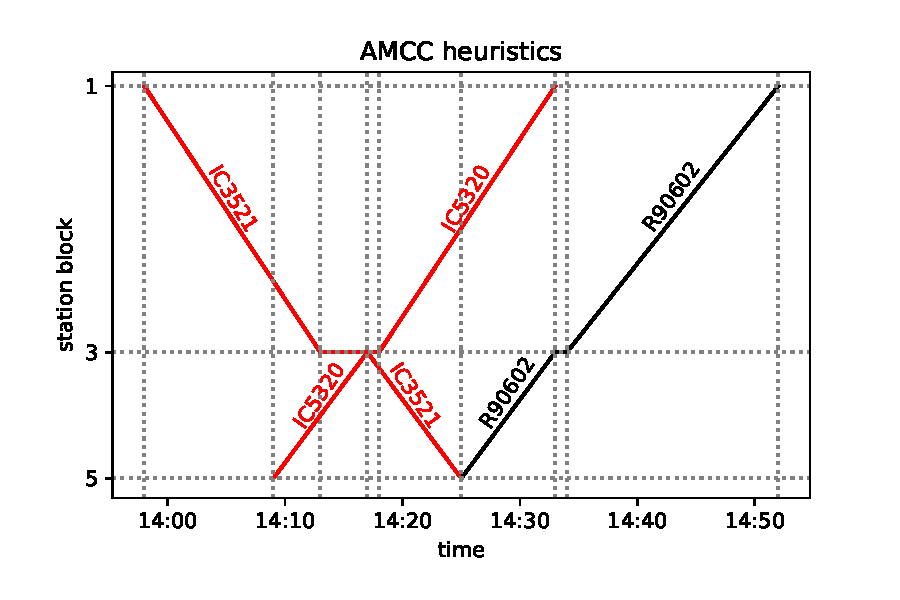
\includegraphics[width=\textwidth]{figures/small_solution}
  \end{subfigure}
  \caption{
    \subref{conflict} Conflicted timetable for railway segment of line No. 216. Compared to the original timetable
    (Fig. \ref{fig:linesmall:diagram}), two trains are delayed, resulting in two conflicts. The conflicts
    can be quickly identified visually as intersections of train paths at line blocks.
    \subref{resolution} Conflict resolution via AMCC heuristics. The same solution was obtained using FCFS and FLFS heuristics.
  }
  \label{fig:smallconflict}
\end{figure}

For the Goleszów -- Wisła Uzdrowisko line, we considered several different
scenarios, which were designed to illustrate our approach on a larger example:

\begin{enumerate}
  \item A moderate delay of the \emph{Inter--City} train starting from the station
    block 1. This results in a single conflict between IC1 and Ks2.
  \item A moderate delay of all the trains starting from station block 1, resulting in
    two conflicts.
  \item A significant delay of some trains starting from station block 1. Results in
    two conflicts.
  \item A significant delay of the \emph{Inter--City} train IC1 starting from the
    station block 1. Results in a single conflict, which is straightforward to
    resolve.
\end{enumerate}

The delays in all the aforementioned scenarios were chosen so that they indeed
result in conflicts. The conflicted timetables are presented in Fig.
\ref{fig:conflictlarge}.

\begin{figure}
  \begin{subfigure}[b]{0.5\textwidth}
    \caption{}\label{c1}
    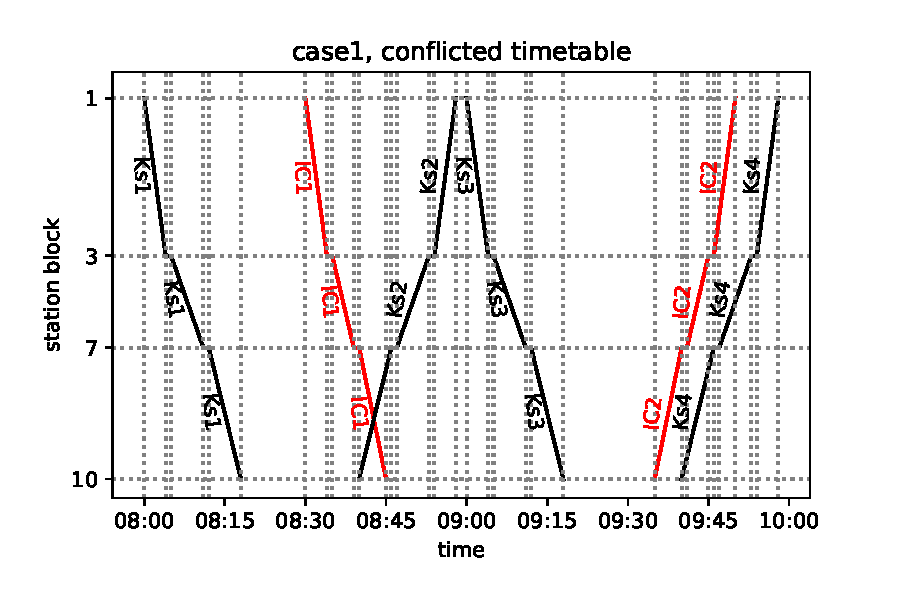
\includegraphics[width=\textwidth]{figures/case1_conflict}
  \end{subfigure}
  \begin{subfigure}[b]{0.5\textwidth}
    \caption{}\label{c2}
    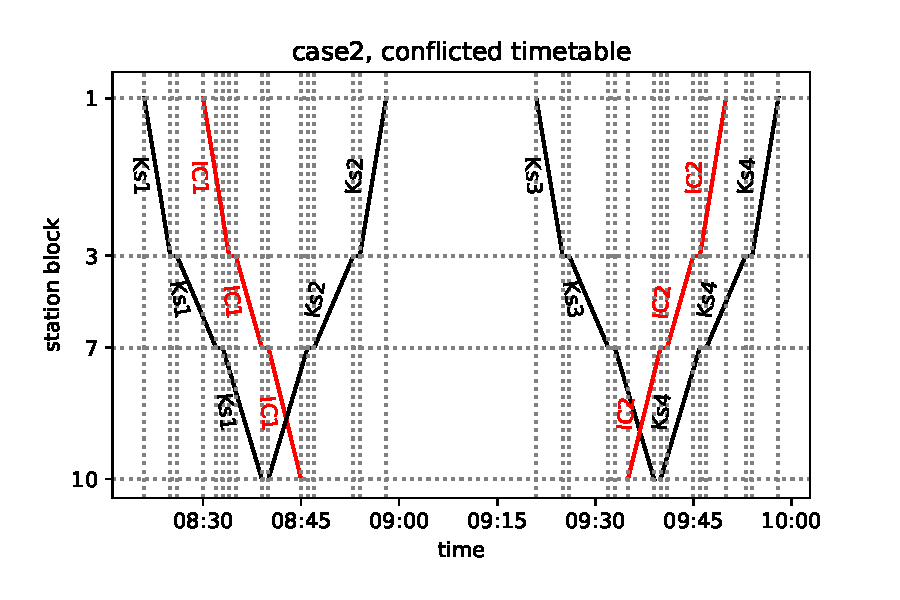
\includegraphics[width=\textwidth]{figures/case2_conflict}
  \end{subfigure}

  \begin{subfigure}[b]{0.5\textwidth}
    \caption{} \label{c3}
    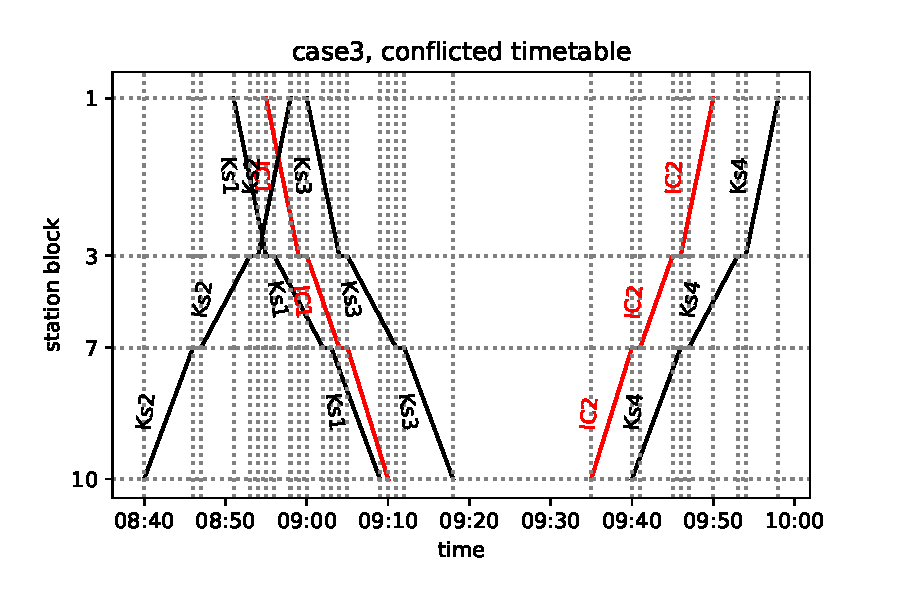
\includegraphics[width=\textwidth]{figures/case3_conflict}
  \end{subfigure}
  \begin{subfigure}[b]{0.5\textwidth}
    \caption{}\label{c4}
    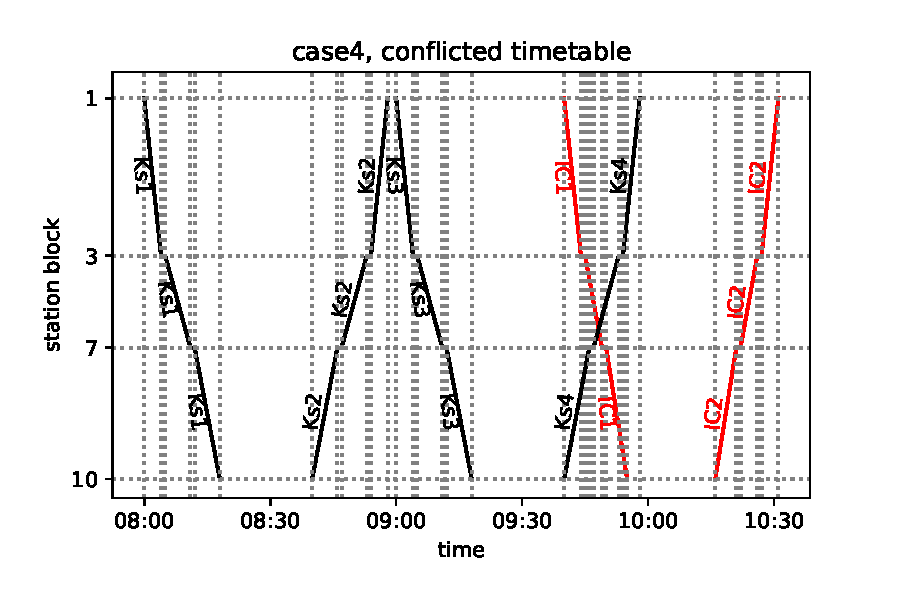
\includegraphics[width=\textwidth]{figures/case4_conflict}
  \end{subfigure}
  \caption{Conflicted timetables for line No. 216. \subref{c1} Single conflict, observe
    that the additional delay of Ks$2$ will propagate to the delay of Ks$3$.
    \subref{c2} Two conflicts, with no impact of Ks$2$ on Ks$3$. \subref{c3}
    Multiple conflicts. \subref{c4} One conflict, straightforward to resolve.}
  \label{fig:conflictlarge}
\end{figure}

\subsection{Solution using simple heuristics}
To establish a baseline for Quantum Annealing, we solved the problems described
in the previous section using simple heuristics common in the railways
practice. Those heuristics are:

\begin{itemize}
  \item FCFS (First Come First Served),
  \item FLFS (First Leave First Served),
  \item AMCC (Avoid Maximum Current $C_{\max}$.
\end{itemize}

In FCFS (resp. FLFS) the way is given to the train that first arrives (resp.
first leaves) the considered station block at which the conflict occurs. AMCC
\cite{mascis2002job} is slightly more complex. In this heuristic, one tries to
minimize the maximum secondary delays of the trains. We want to stress that
those heuristics facilitate different objective functions, and hence it is not
possible to directly compare them -- nevertheless, it might be useful to
discuss qualitative differences between the solutions they produce. The
solutions provided by the AMCC heuristic also provide a lower bound for the
values of maximum secondary delays $d_{\max}(j)$, which we will use when
constructing QUBO.

For the case of Nidzica--Olsztynek line, all heuristics returned the same
solution, depicted in Fig. \ref{resolution}. The conflict is avoided by
delaying IC3521 by another 3-minutes, and allowing R9062 to enter the block not
earlier than 14:25, i.e. 4 minutes later than in the conflicted timetable. In
this case, the additional 4 minutes constitute the maximum secondary delay of
the solution.

We also applied the aforementioned heuristics to all the considered
disturbances in the Goleszów -- Wisła Uzdrowisko segment. For brevity, we
refrain from presenting a detailed discussion of the solutions for all the
cases and limit ourselves to the summary of the maximum secondary delay, which
is presented in Table \ref{tab:simple}

\begin{table}[bh]
  \centering
  \begin{tabular}{|c|c|c|c|c|}
    \hline
    \rowcolor{theader} Heuristics & case $1$ & case $2$ & case $3$ & case $4$ \\
    \hline
    FLFS       & 6        & 13       & 4        & 2        \\
    \hline
    FCFS       & 5        & 5        & 5        & 2        \\
    \hline
    AMCC       & 5        & 5        & 4        & 2        \\
    \hline
  \end{tabular}
  \caption{The maximum secondary delays, in minutes, resulting from simple heuristics.
    Observe that for each case, there are solutions far below $d_{\text{max}} =
      10$.} \label{tab:simple}
\end{table}

\subsection{Details on QUBO construction}

To formulate our dispatching problems as QUBO and solve them on the D-Wave
annealer (or using any other method), we first need to decide on the values of
several parameters of the model, as well as the precise form of the cost
function. We start with the latter.

We decided on using the cost function proportional to the secondary delays of
all trains entering their last station block. Additionally, we weight the
contributions of each delay with a coefficient depending on the prioritization
of the corresponding train, resulting in the cost function of the form:
\begin{equation}
  f(\mathbf{x}) = \sum_{j \in J}\left(\sum_{m  \in A_{j,s^{*}}}w_{j} \frac{d(j,s^{*}) - d_{U}(j,s^{*})}{d_{\max}(j)}x_{j,s^{*},m}\right),
\end{equation}
where $s^{*} = s_{j,end-1}$. The priorities $w_{j}$ are chosen specifically for
both networks. One can immediately observe that larger values of $w_{j}$
increase contribution stemming from the delay of a given train, and hence the
objective function favors solutions with smaller delays for the trains with
larger priorities. For the segment of line No. 216, we assume $w_{j}= 1.5$ for
all \emph{Inter-City} trains, and the $w_{j}=1.0$ for the regional train. This
prioritization coincides with the usual prioritization of trains in Poland (and
many countries). For the segment of line No. 191, we decided to adopt a
slightly more complicated prioritization. For the trains heading toward block
10, we set a lower priority of $w_{j}=0.9$. For the trains heading in the
opposite direction, we set $w_{j}=1.5$ and $w_{j}=1.0$ for \emph{Inter-City}
and regional trains respectively. This is because the trains heading towards
block 1 (Goleszów) also head towards important junctions in Polish railway
network (Katowice for regional trains, and capital city of Warsaw for
\emph{Inter-city} trains). Our strategy therefore tries to avoid larger delays
in this direction to limit further disturbance to the rest of the network.

As for the maximum secondary delay $d_{\max}$, for simplicity, we assume it is
the same for all trains. On the one hand, its value cannot be smaller than the
one returned by the AMCC heuristics. On the other hand, setting this value too
high increases the number of decision variables and complicates the objective
function, which is especially undesirable because of the limited number of
qubits on D-Wave annealers. For line No. 216, we set $d_{\max}=7$ and for line
No. 191 we set $d_{\max}=10$. The total number of decision variables is given
by
\begin{equation}
  \mbox{\#variables} = (\mbox{\#station blocks}-1) \cdot (\mbox{\#number of trains}) \cdot (d_{\max}+1)
\end{equation}
We therefore get $2\cdot 3 \cdot 8 = 48$ decision variables for line No. 216
and $3 \cdot 6 \cdot 11 = 198$ variables for line No. 191. Importantly, the
moderately low number of variables for line no. 216 allows us to solve it using
the brute--force algorithm presented in Chapter \ref{chapter:bruteforce}.

Lastly, we need to choose values for $p_{pair}$ and $p_{sum}$ penalty weights.
This is a very subtle choice. On the one hand, setting it too low may cause
some of the infeasible solutions to have the value of the objective function
smaller than that of feasible solutions, which is undesirable. On the other
hand, if penalty weights are too high, the actual cost function becomes merely
a perturbation for the penalty terms, which is also undesirable. To illustrate
the difference those weights make to the energy landscape, we computed the
low-energy spectrum for the problem defined on line No. 216 for several
different values of $p_{pair}$ and $p_{sum}$. The histograms of energies
obtained in this way are presented in Fig. \ref{fig:penaltyhistogram}.

\begin{figure}
  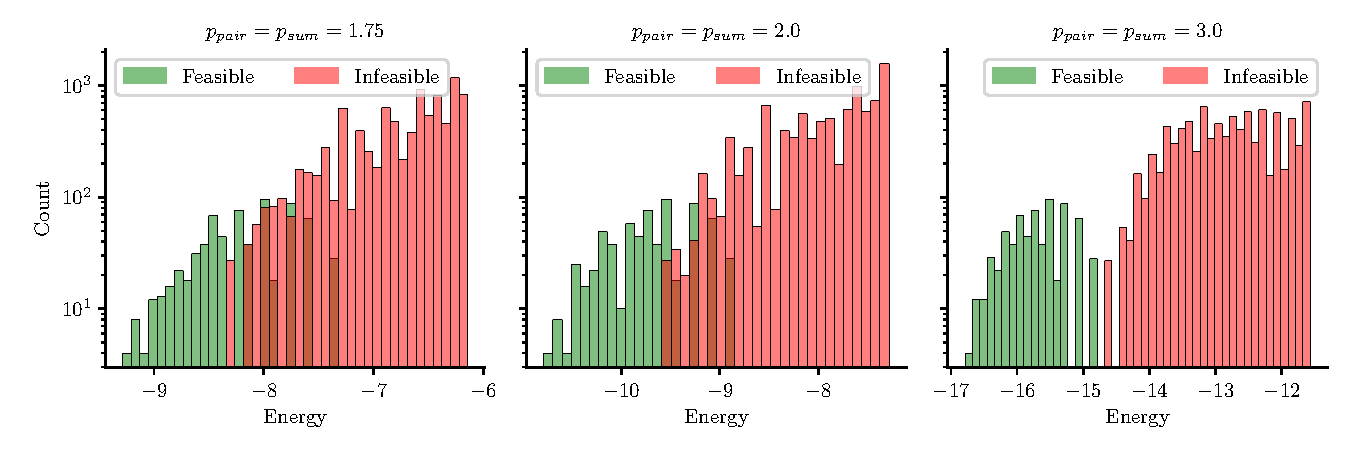
\includegraphics[width=\textwidth]{figures/railway_histograms_bf}
  \caption{Energy histogram for feasible (green) and infeasible (red) solutions of QUBO
    defined for line No. 216 with varying penalty weights. The figure takes into
    account first 5000 low energy states.} \label{fig:penaltyhistogram}
\end{figure}
In our experiments, we used several combinations of $p_{pair}$ and $p_{sum}$.

\subsubsection{Solutions using the D-Wave annealer}

All QUBOs presented in this chapter have a small number of variables relative
to the number of qubits available in the current generation of the annealers.
The density of the graphs, defined as the number of edges relative to the
number of edges in a full graph with the same number of vertices, is also
relatively low. Nevertheless, the problem graphs are not compatible with the
topology of the current generation of the annealers and hence had to be
embedded. We used several chain strengths in our experiments, ranging from $4$
to $12$, with those values being determined by running a set of initial samples
and assessing the results. Similarly, we also used several values of annealing
time $\\tau$ ranging from $5$ to $2000$.

The problem defined on Line 216 was small enough to fit on all devices,
including two Pegasus-based Advantage systems and a new prototype Advantage2
system featuring Zephyr topology. All of the annealers were able to find a
feasible solution to the problem for at least some combination of parameters.
However, their performance varied highly depending on the parameter range. The
frequency of finding a feasible solution by the annealers is depicted in Fig.
\ref{fig:dwline216freq}. As seen there, the Advantage system6.3 and Advantage2
prototype1.1 devices exhibited much better performance than the older Advantage
system4.1 device. As for the quality of the solutions, all solvers managed to
find an optimal solution, although with different frequencies. The summary of
parameters for which a ground state was obtained is presented in table
\ref{tab:line216ground}. Example ground states found are depicted in Fig.
\ref{fig:dwline216grounds}.

\begin{table}
  \small
  \centering
  \begin{tabular}{|c|c|c|c|}
    \hline
    \rowcolor{theader} Solver & chain strength & annealing time & \# occurrences \\
    \hline
    Advantage System4.1       & 10             & 200            & 1              \\
    \hline
    Advantage System4.1       & 12             & 500            & 1              \\
    \hline
    \hline
    Advantage System6.3       & 10             & 500            & 1              \\
    \hline
    Advantage System6.3       & 12             & 100            & 1              \\
    \hline
    \hline
    Advantage2 Prototype1.1   & 12             & 5              & 1              \\
    \hline
    Advantage2 Prototype1.1   & 12             & 100            & 3              \\
    \hline
    Advantage2 Prototype1.1   & 12             & 1000           & 4              \\
    \hline
    Advantage2 Prototype1.1   & 12             & 2000           & 1              \\
    \hline
  \end{tabular}
  \caption{Parameters for which D-Wave annealer managed to find the optimal solution to
    the problem defined on Line 216. All ground states occurred at
    $p_{\text{pair}}=p_{\text{sum}}=4.0$. } \label{tab:line216ground}
\end{table}

\begin{figure}[b]
  \begin{subfigure}[b]{0.5\textwidth}
    \caption{}\label{c1}
    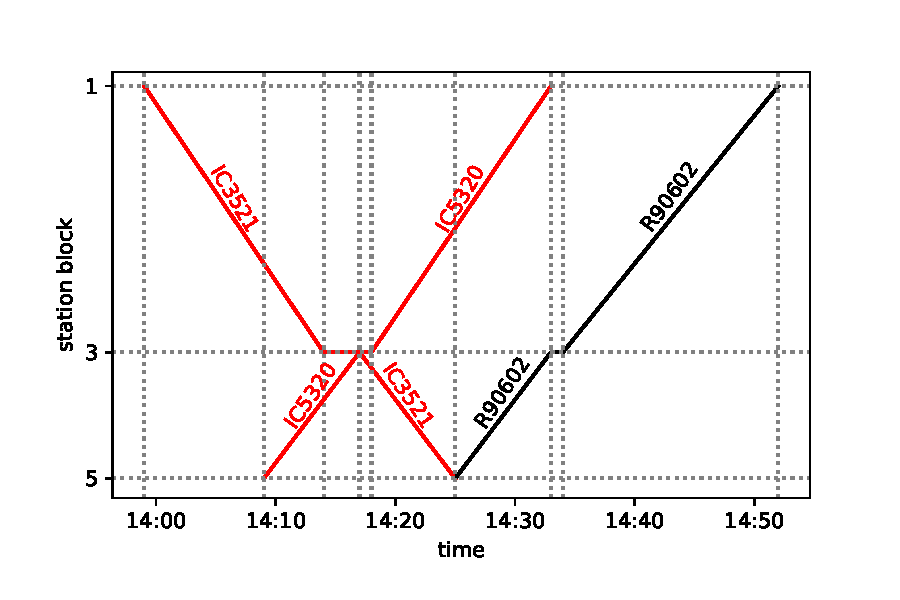
\includegraphics[width=\textwidth]{figures/dwave_line216_ground1}
  \end{subfigure}
  \begin{subfigure}[b]{0.5\textwidth}
    \caption{}\label{c2}
    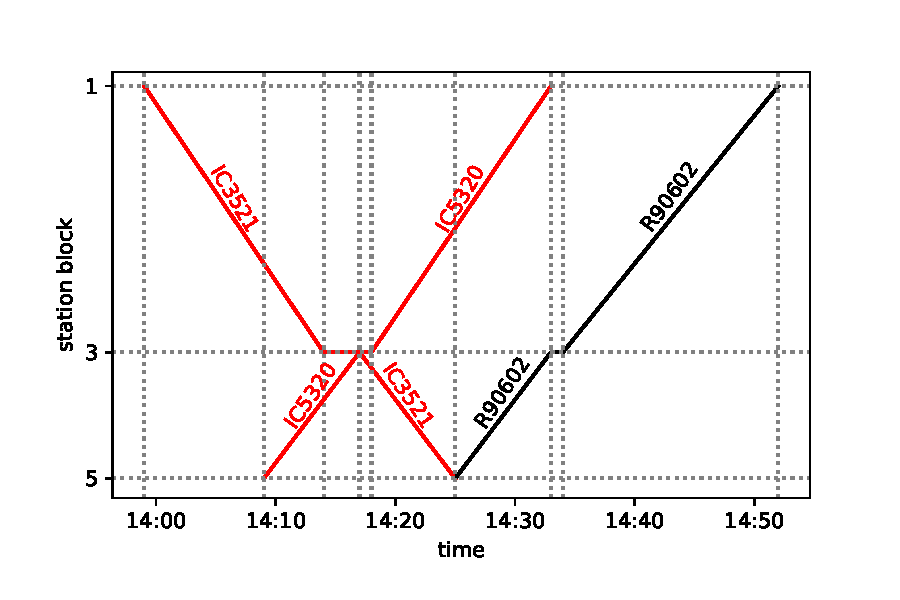
\includegraphics[width=\textwidth]{figures/dwave_line216_ground1.pdf}
  \end{subfigure}
  \caption{Example ground state solutions for the conflicted timetable of Line 216. All
    other ground states are equivalent from the dispatching point of view.}
  \label{fig:dwline216grounds}
\end{figure}

\begin{figure}
  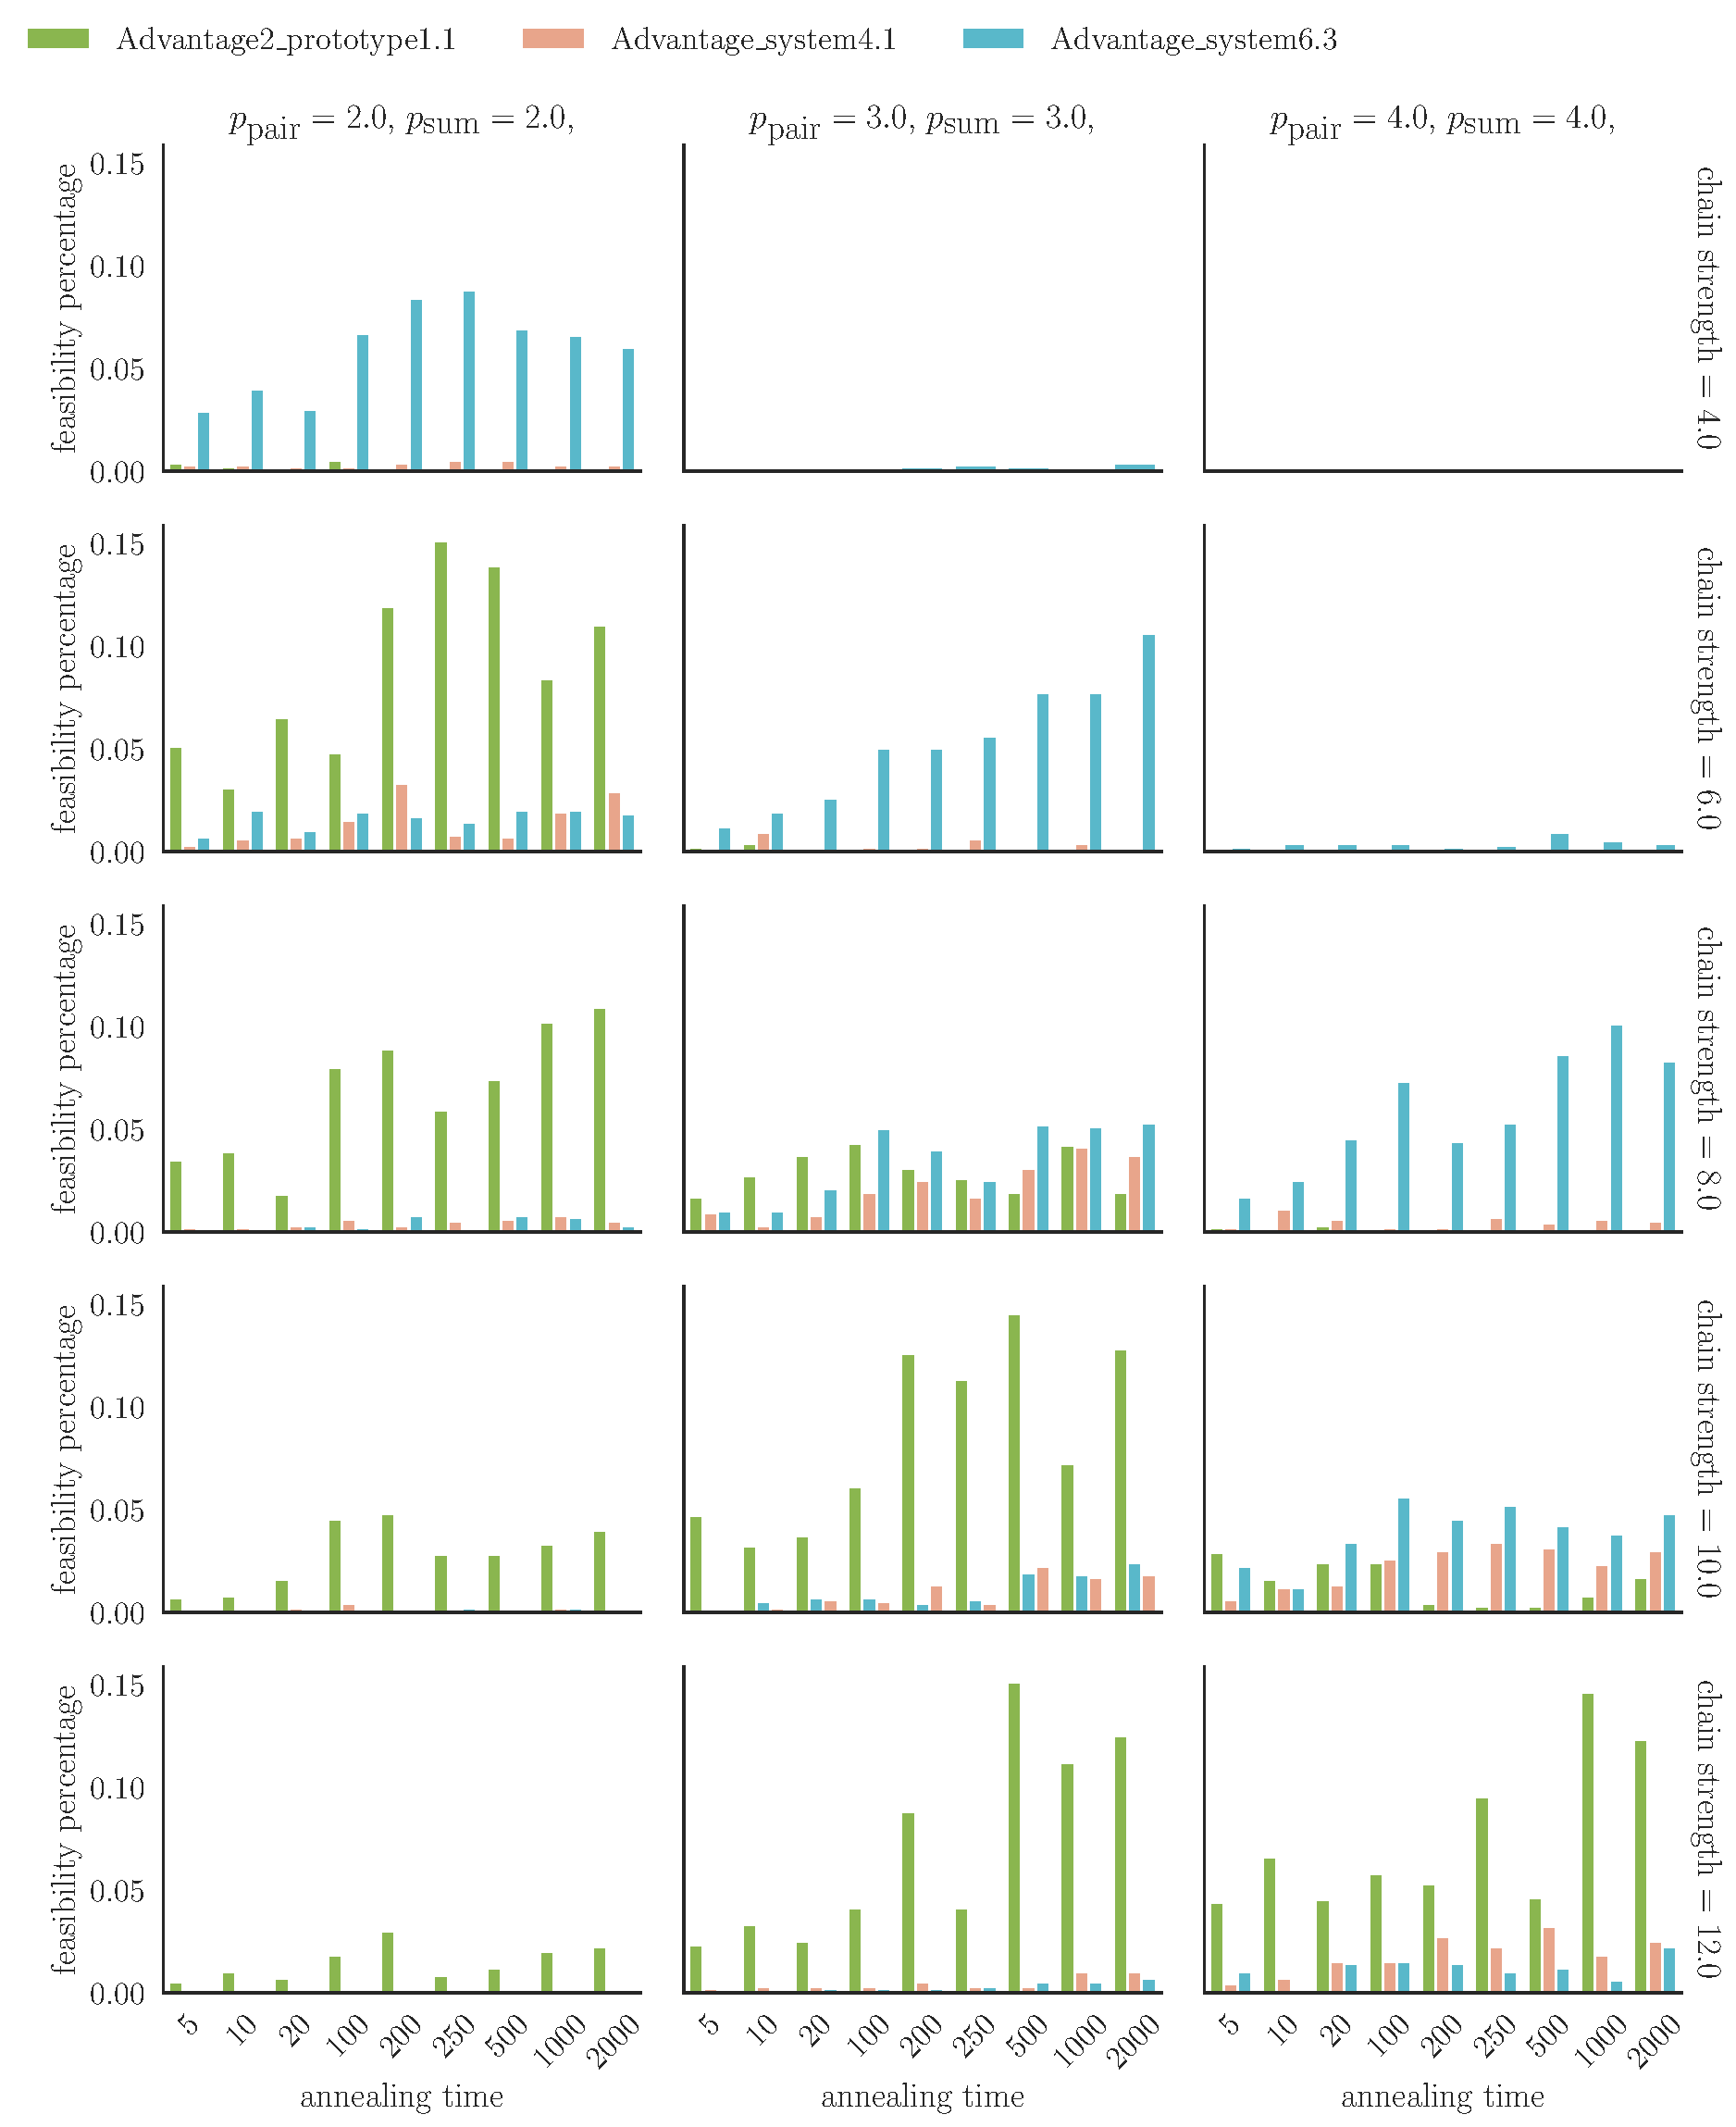
\includegraphics[width=\textwidth]{figures/dwave_line_216_result.pdf}
  \caption{
    Frequency of finding a feasible solution for the problem defined for Line 216.
    Rows in the grid correspond to different values of chain strength and the
    columns correspond to different values of penalty scalings. In each cell, the
    X-axis depicts the annealing time $\tau$, while the $Y$-axis depicts the
    obtained fraction of the feasible solution (out of 1000 samples) }
  \label{fig:dwline216freq}
\end{figure}

%%% Local Variables:
%%% mode: pdflatex
%%% TeX-master: "../main"
%%% End:
